\newpage
\section{Auswertung}
\label{sec:Auswertung}

\subsection{Bestimmung der Güteziffer}

\subsubsection{Aufg. a: Messdaten und Diagramm}

Die gemessenen Daten werden wie folgt tabellarisch dargestellt. 

\begin{table}
  \centering
  \caption{Messdaten}
  \label{tab:Messdaten}
  %\sisetup{table-format=1.2}
  %\resizebox{.5/textwidth}{!}{%
  \begin{tabular}{c c c c c c c}  %\begin{tabular}{S[table-format=3.0] c c c c c c c[table-format=3.2]}
    \toprule
    {$t (\unit{\second})$} &
    {$T_{1} (\unit{\celsius})$}&
    {$T_{2} (\unit{\celsius})$}&
    {$p_{a} (\unit{\bar})$}&
    {$p_{b} (\unit{\bar})$}&
    {$P (\unit{\watt})$} \\
    \midrule
       0 &    21.50 &     21.50 &       4.20 &       3.80 &      - \\
      60 &    23.30 &     20.70 &       3.90 &       5.30 &      - \\
     120 &    24.70 &     19.30 &       3.60 &       5.90 &      - \\
     180 &    26.40 &     17.70 &       3.60 &       6.00 &      - \\
     240 &    27.90 &     16.60 &       3.60 &       6.40 &      - \\
     300 &    29.50 &     15.60 &       3.50 &       6.80 & 125.00 \\
     360 &    31.00 &     14.60 &       3.30 &       7.00 & 125.00 \\
     420 &    32.50 &     13.50 &       3.20 &       7.40 & 125.00 \\
     480 &    33.80 &     12.50 &       3.00 &       7.50 & 125.00 \\
     540 &    35.10 &     11.50 &       2.40 &       8.00 & 125.00 \\
     600 &    36.20 &     10.60 &       2.80 &       8.10 & 125.00 \\
     660 &    37.50 &      9.60 &       2.70 &       8.50 & 125.00 \\
     720 &    38.50 &      8.70 &       2.80 &       8.90 & 125.00 \\
     780 &    39.60 &      7.80 &       2.50 &       9.00 & 125.00 \\
     840 &    40.60 &      7.10 &       2.40 &       9.10 & 115.00 \\
     900 &    41.50 &      6.20 &       2.40 &       9.30 & 115.00 \\
     960 &    42.40 &      5.50 &       2.20 &       9.70 & 115.00 \\
    1020 &    43.30 &      4.70 &       2.10 &       9.90 & 115.00 \\
    1080 &    44.10 &      4.00 &       2.10 &      10.10 & 115.00 \\
    1140 &    44.80 &      3.30 &       2.10 &      10.20 & 115.00 \\
    1200 &    45.60 &      2.70 &       2.00 &      10.50 & 115.00 \\
    1260 &    46.30 &      2.10 &       2.00 &      10.80 & 115.00 \\
    1320 &    47.10 &      1.40 &       1.90 &      11.00 & 115.00 \\
    1380 &    47.80 &      0.80 &       1.80 &      11.10 & 115.00 \\
    1440 &    48.40 &      0.30 &       1.80 &      11.20 & 115.00 \\
    1500 &    49.00 &     -0.20 &       1.80 &      11.60 & 115.00 \\
    1560 &    49.50 &     -0.70 &       1.80 &      11.80 & 115.00 \\
    1620 &    50.00 &     -0.10 &       1.80 &      12.00 & 115.00 \\
    \bottomrule
  \end{tabular}
\end{table}

\newpage
Alle Größen wurden in SI-Einheiten umgerechnet, die Temperatur zudem invers dargestellt,
die Zeit für die Ausgleichsrechnung quadriert und gemäß der Versuchsanleitung \cite{v206} den Drücken $\textit{p}_\textit{a}$ und $\textit{p}_\textit{b}$ 1 bar bzw. 100000 Pa addiert:

\begin{table}
  \centering
  \caption{Messdaten}
  \label{tab:berechnete_werte}
  %\sisetup{table-format=1.2}
  %\resizebox{.5/textwidth}{!}{%
  \begin{tabular}{c c c c c c}  %\begin{tabular}{S[table-format=3.0] c c c c c c c[table-format=3.2]}
    \toprule
    {$t^{2} (\unit{\second\squared})$}&
    {$T_{1} (\unit{\kelvin})$}&
    {$T_{2} (\unit{\kelvin})$}&
    {$p_{a+} (\unit{\pascal})$}&
    {$p_{b+} (\unit{\pascal})$}&
    {$1/T_{1} (1/\unit{\kelvin})$} \\
    \midrule
          0.00 &  294.65 &  294.65 & 520000.00 &  480000.00 &      0.0034 \\
       3600.00 &  296.45 &  293.85 & 490000.00 &  630000.00 &      0.0034 \\
      14400.00 &  297.85 &  292.45 & 460000.00 &  690000.00 &      0.0034 \\
      32400.00 &  299.55 &  290.85 & 460000.00 &  700000.00 &      0.0033 \\
      57600.00 &  301.05 &  289.75 & 460000.00 &  740000.00 &      0.0033 \\
      90000.00 &  302.65 &  288.75 & 450000.00 &  780000.00 &      0.0033 \\
     129600.00 &  304.15 &  287.75 & 430000.00 &  800000.00 &      0.0033 \\
     176400.00 &  305.65 &  286.65 & 420000.00 &  840000.00 &      0.0033 \\
     230400.00 &  306.95 &  285.65 & 400000.00 &  850000.00 &      0.0033 \\
     291600.00 &  308.25 &  284.65 & 340000.00 &  900000.00 &      0.0032 \\
     360000.00 &  309.35 &  283.75 & 380000.00 &  910000.00 &      0.0032 \\
     435600.00 &  310.65 &  282.75 & 370000.00 &  950000.00 &      0.0032 \\
     518400.00 &  311.65 &  281.85 & 380000.00 &  990000.00 &      0.0032 \\
     608400.00 &  312.75 &  280.95 & 350000.00 & 1000000.00 &      0.0032 \\
     705600.00 &  313.75 &  280.25 & 340000.00 & 1010000.00 &      0.0032 \\
     810000.00 &  314.65 &  279.35 & 340000.00 & 1030000.00 &      0.0032 \\
     921600.00 &  315.55 &  278.65 & 320000.00 & 1070000.00 &      0.0032 \\
    1040400.00 &  316.45 &  277.85 & 310000.00 & 1090000.00 &      0.0032 \\
    1166400.00 &  317.25 &  277.15 & 310000.00 & 1110000.00 &      0.0032 \\
    1299600.00 &  317.95 &  276.45 & 310000.00 & 1120000.00 &      0.0031 \\
    1440000.00 &  318.75 &  275.85 & 300000.00 & 1150000.00 &      0.0031 \\
    1587600.00 &  319.45 &  275.25 & 300000.00 & 1180000.00 &      0.0031 \\
    1742400.00 &  320.25 &  274.55 & 290000.00 & 1200000.00 &      0.0031 \\
    1904400.00 &  320.95 &  273.95 & 280000.00 & 1210000.00 &      0.0031 \\
    2073600.00 &  321.55 &  273.45 & 280000.00 & 1220000.00 &      0.0031 \\
    2250000.00 &  322.15 &  272.95 & 280000.00 & 1260000.00 &      0.0031 \\
    2433600.00 &  322.65 &  272.45 & 280000.00 & 1280000.00 &      0.0031 \\
    2624400.00 &  323.15 &  273.05 & 280000.00 & 1300000.00 &      0.0031 \\
    \bottomrule
  \end{tabular}
\end{table}

\newpage


Im Folgenden werden die Temperaturverläufe in einem Diagramm dargestellt:

\begin{figure}
  \centering
  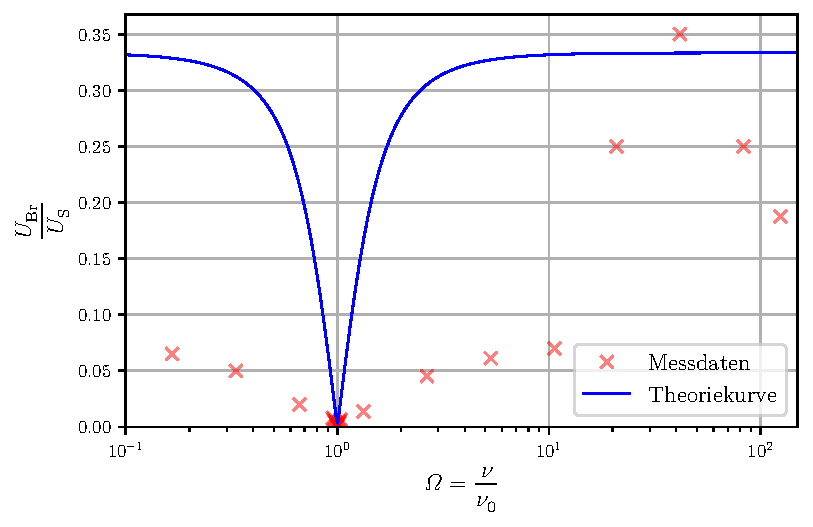
\includegraphics{plot.pdf}
  \caption{Temperaturverläufe während der Messung}
  \label{fig:plot}
\end{figure}

\subsubsection{Aufg. b: Bestimmung der Parameter der Näherungsfunktion}

Eine nicht-lineare Ausgleichsrechnung der Temperaturverläufe mittels PYTHON mithilfe der Näherungsfunktion

\begin{equation} 
  T(t) = At^2 + Bt + C 
\end{equation}
\\
ergibt die folgenden Parameter für $T_{1} (\unit{\kelvin})$: \\
A = \qty{-6.6217(1407)e-6}{\unit[per-mode=reciprocal]{\kelvin\per\second\squared}} \\
B = \qty{0.0281(0002)}{\unit[per-mode=reciprocal]{\kelvin\per\second}} \\
C = \qty{294.7858(0.0825)}{\unit\kelvin} \\
\\
und für $T_{2} (\unit{\kelvin})$: \\
A = \qty{4.6346(1811)e-6}{\unit[per-mode=reciprocal]{\kelvin\per\second\squared}} \\
B = \qty{-0.0214(0003)}{\unit[per-mode=reciprocal]{\kelvin\per\second}} \\
C = \qty{294.8097(0.1062)}{\unit\kelvin} \\



% quadratische regression für T_1 und T_2

\subsubsection{Aufg. c: Bestimmung der Differentialquotienten}

% usepackage{}